\documentclass[alsotrans]{beamerswitch}
\usepackage{fprog}

\title[Какво е ФП?]{Какво е функционално програмиране?}

\newcommand{\lang}[1]{\onslide<2->{\hspace{2ex}[\textbf{#1}]}}
\newcommand{\scheme}{\lang{Scheme}}
\newcommand{\haskell}{\lang{Haskell}}

\date{2 октомври 2019 г.}

\begin{document}

\begin{frame}
  \titlepage
\end{frame}

\section*{Императивен и декларативен стил}

\begin{frame}
  \frametitle{Императивен стил}

  Описваме последователно изчислителните стъпки.\\[1em]
  \begin{columns}[t,onlytextwidth]

    \column{0.5\textwidth}
    \textbf{Неструктурирано\\програмиране}\\[1em]
    \begin{enumerate}
    \item Въведи \tt a, \tt b
    \item Ако \tt{a $=$ b}, към 6.
    \item Ако \tt{a $>$ b}, към 5.
    \item \tt{b $\leftarrow$ b $-$ a}; към 2.
    \item \tt{a $\leftarrow$ a $-$ b}; към 2.
    \item Изведи a
    \item Край
    \end{enumerate}

    \column{0.5\textwidth}
    \textbf{Структурирано\\програмиране}\\[1em]
    \begin{itemize}
    \item Въведи \tt a, \tt b
    \item Докато \tt{a $\neq$ b}
      \begin{itemize}
      \item Ако \tt{a $>$ b}
        \begin{itemize}
        \item \tt{a $\leftarrow$ a $-$ b}
        \end{itemize}
      \item В противен случай
        \begin{itemize}
        \item \tt{b $\leftarrow$ b $-$ a}
        \end{itemize}
      \end{itemize}
    \item Изведи \tt a
    \end{itemize}

  \end{columns}
\end{frame}

\begin{frame}
  \frametitle{Декларативен стил}

  Описваме свойствата на желания резултат.\\[1em]
  \textbf{Програмиране с ограничения}
  \begin{itemize}
  \item Дадени са \tt a и \tt b.
  \item Търсим \tt d, такова че:
    \begin{itemize}
    \item \tt{1 $\leq$ d $\leq$ a,b}
    \item ``\tt d е делител на \tt a''
    \item ``\tt d е делител на \tt b''
    \item \tt d е възможно най-голямо,
    \item където за дадени \tt x и \tt y:
      \begin{itemize}
      \item ``\tt x е делител на \tt y'', ако
      \item намерим такова естествено число \tt k, че
      \item \tt{1 $\leq$ k $\leq$ y}
      \item \tt k * \tt x = \tt y
      \end{itemize}
    \end{itemize}
  \end{itemize}
\end{frame}

\begin{frame}
  \frametitle{Декларативен стил (2)}

  Описваме свойствата на желания резултат.\\[1em]
  \textbf{Логическо програмиране}
  \begin{itemize}
  \item Описваме релацията над естествени числа $gcd(a,b,c)$
  \item $\forall a \, gcd(a,a,a)$ \hspace{2ex}\textbf{[факт]}
  \item $\forall a\forall b ( a > b \land \forall c (gcd(a-b,b,c) \rightarrow gcd(a,b,c)))$ \hspace{2ex}\textbf{[правило 1]}
  \item $\forall a\forall b ( a < b \land \forall c (gcd(a,b-a,c) \rightarrow gcd(a,b,c)))$ \hspace{2ex}\textbf{[правило 2]}
  \item Дадени са $a, b$
  \item Намери такова $c$, за което $gcd(a,b,c)$
  \end{itemize}
  \pause
  \textbf{Пример:}
  Нека $a = 8, b = 12$. Тогава:\\
  $\xrightarrow{\text{факт}} gcd(4,4,4) \xrightarrow{\text{правило 1}} gcd(8,4,4) \xrightarrow{\text{правило 2}} gcd(8,12,\mathbf4)$
\end{frame}


\begin{frame}
  \frametitle{Декларативен стил (3)}
  Описваме свойствата на желания резултат.\\[1em]
  \textbf{Функционално програмиране}
  \begin{itemize}
  \item Функцията над естествени числа $gcd(a,b)$ притежава следните свойства:
  \item $gcd(a,a) = a$ \hspace{2ex}\textbf{(свойство 1)}
  \item $gcd(a-b,b) = gcd(a,b)$, ако $a > b$ \hspace{2ex}\textbf{(свойство 2)}
  \item $gcd(a,b-a) = gcd(a,b)$, ако $b > a$ \hspace{2ex}\textbf{(свойство 3)}
  \item Дадени са $a, b$
  \item Да се пресметне $gcd(a,b)$.
  \end{itemize}
  \pause
  \textbf{Пример:}
  Нека $a = 8, b = 12$.\\
  $gcd(8,12) \stackrel{\text{свойство 3}}= gcd(8,4) \stackrel{\text{свойство 2}}= gcd(4,4) \stackrel{\text{свойство 1}}= 4$.
\end{frame}

\begin{frame}
  \frametitle{Още един пример}

  Да се намери сумата на квадратите на нечетните числа в списъка \tt l.\\[1em]
  \begin{columns}[t,onlytextwidth]
    \column{0.5\textwidth}
    \textbf{Императивен стил}
    \begin{itemize}
    \item Нека \tt{s = 0}.
    \item За \tt i от 1 до \tt{length(l)}:
      \begin{itemize}
      \item Ако \tt{l[i]} е нечетно, то
        \begin{itemize}
        \item \tt{s = s + l[i]$^2$}.
        \end{itemize}
      \end{itemize}
    \item Изведи \tt s.
    \end{itemize}

    \column{0.5\textwidth}
    \textbf{Функционален стил}
    \begin{itemize}
    \item От елементите на \tt l\ldots
    \item \ldots избираме нечетните, \ldots
    \item \ldots прилагаме над тях функцията $x^2$ \ldots
    \item \ldots и ги групираме с операцията $+$.
    \end{itemize}
  \end{columns}
\end{frame}

\begin{frame}[fragile]
  \frametitle{Още един пример (2)}
  \textbf{C++:}
\begin{verbatim}
int s = 0;
for(int i = 0; i < sizeof(l); i++)
  if (l[i] % 2 != 0)
    s += l[i] * l[i];
cout << s;
\end{verbatim}
  \pause
  \textbf{Scheme:} \tt{(apply + (map square (filter odd? l)))}\\[1em]
  \pause
  \textbf{Haskell:} \tt{foldr1 (+) [ x\^{}2 | x <- l, odd x ]}\\[1em]
  \pause
  \textbf{Haskell:} \tt{sum . map (\^{}2) . filter odd}
\end{frame}

\section*{Изчислителни модели}

\begin{frame}
  \frametitle{Какво може да се сметне с компютър?}

  Нека $f:\mathbb N\to\mathbb N$ е функция над естествени числа.\\[1em]

  \textbf{Примери:} $f(x) = x^2$, $f(x) = x$-тото число на Фибоначи.\\[2em]
  \pause
  \textbf{Въпрос 1:} Какво означава да изчислим $f$ с компютър?\\[2em]
  \pause
  \textbf{Въпрос 2:} Какво означава ``алгоритъм'' или ``програма''?\\[2em]
  \pause
  \textbf{Въпрос 3:} Има ли функции, които не могат да бъдат изчислени с компютър?
\end{frame}

\begin{frame}
  \frametitle{Машина на Turing}

  % TODO: да се нарисува с TikZ
  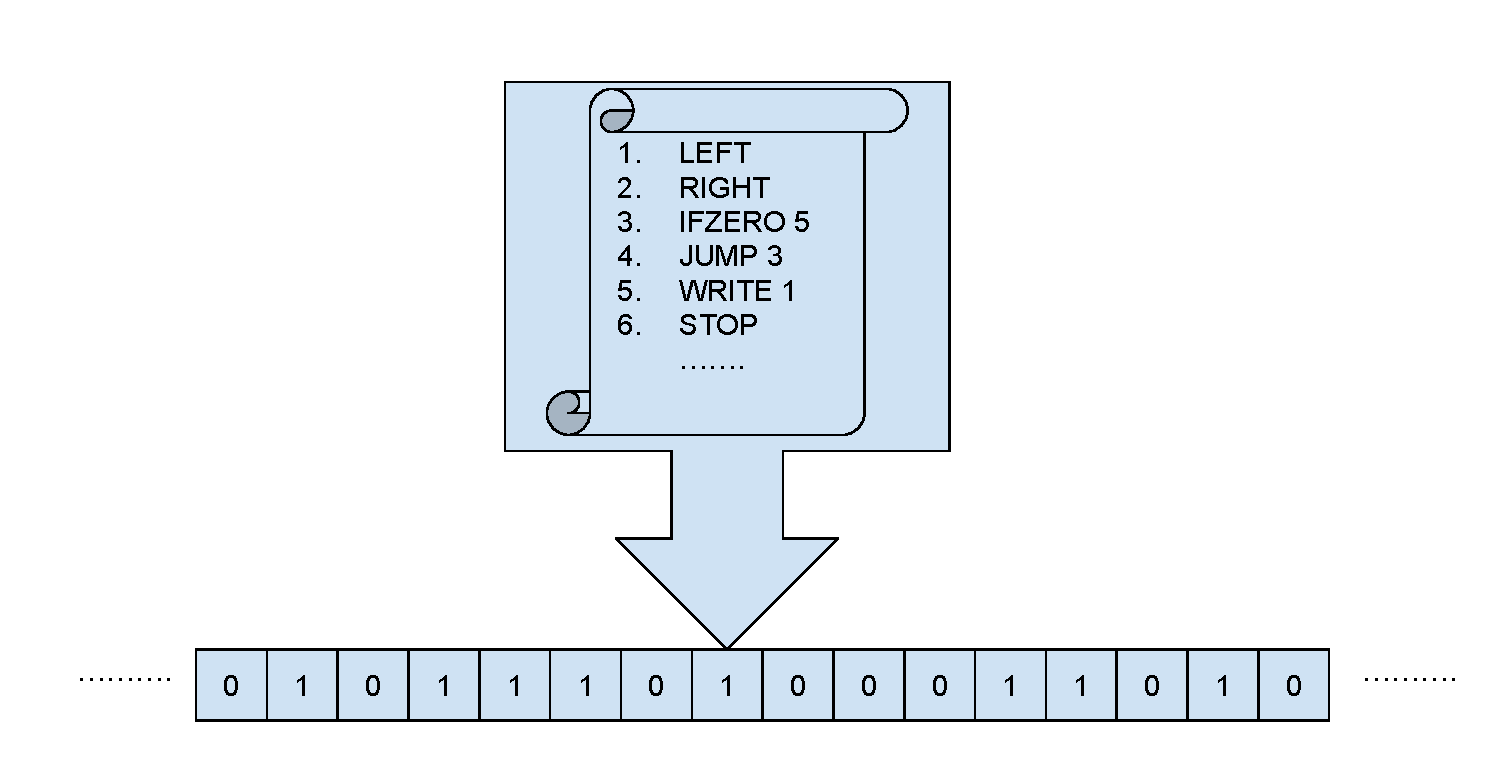
\includegraphics[width=0.9\textwidth]{images/turing.pdf}\\
  \pause
  \textbf{$M$ изчислява функцията $f_M$}, ако при лента с числото $n$ машината $M$ завършва и записва върху лентата числото $f_M(n)$.\\
  \pause
  Ако $M$ не завърши за някое $n$, казваме, че \textbf{$f_M(n)$ не е дефинирана}.
\end{frame}

\begin{frame}
  \frametitle{Има неизчислими функции!}

  \begin{itemize}[<+->]
  \item Всяка машина на Turing може да се кодира като дълго естествено число.
  \item Всяка изчислима функция се изчислява от (поне една) машина.
  \item Следователно, изчислимите функции са не повече от естествените числа (изброимо много).
  \item Но функциите от вида $\mathbb N \to \mathbb N$ са колкото редиците от естествени числа
\ldots
  \item \ldots които са неизброимо много! (защо?).
  \item Следователно, има неизброимо много неизчислими функции. \qed
  \item \alert{Но кои са те?}
  \end{itemize}
\end{frame}

\begin{frame}
  \frametitle{Стоп проблем}

  \small
  Нека с $\mt n$ означаваме машината на Turing с код $n$.\\
  Разглеждаме функцията:
  \begin{equation*}
    halts(n) =
    \begin{cases}
      1,&\text{ ако }\mt n\text{ завършва над лента с числото }n,\\
      0,&\text{ иначе}.
    \end{cases}
  \end{equation*}
  \pause
  \alert{$halts$ не е изчислима!}\\
  \pause
  \begin{proof}
    Да допуснем, че $halts$ се изчислява от машина на Turing $H$.\\
    Дефинираме нова машина на Turing $D$:\\
    \setlength{\leftmargini}{30pt}
    \begin{enumerate}
      \setbeamertemplate{enumerate items}[default]
    \item (тук слагаме всички инструкции на $H$)
    \item[$k+1$.] \tt{IFZERO} $k+3$
    \item[$k+2$.] \tt{JUMP} $k+1$
    \item[$k+3$.] \tt{STOP}
    \end{enumerate}
    Нека $D = \mt d$. Завършва ли $D$ над $d$?
  \end{proof}
\end{frame}

\begin{frame}
  \frametitle{Въпроси за изчислимост}

  Според вас изчислими ли са следните функции?
  \begin{itemize}[<+->]
  \item $f_1(n) = n$ е просто число
  \item $f_2(n) = n$-тото поред просто число
  \item $f_3(n) = n$-тата цифра на числото $\pi$
  \item $f_4(n) = $ има $n$ последователни седмици в числото $\pi$
  \item $f_5(n) = n$ е код на множество от матрици $3 \times 3$, които могат да се умножат в някакъв ред, така че да се получи O
  \item $f_6(n) = n$ е код на вярна съждителна формула
  \item $f_7(n) = n$ е код на вярна предикатна формула
  \item $f_8(n) = m$, където $\mt m$ пресмята $f_8$
  \item $f_9(n) = $ машините $\mt n$ и $\mt{2n}$ изчисляват еднакви функции
  \end{itemize}
\end{frame}

\begin{frame}
  \frametitle{$\lambda$-смятане}

  Нека разполагаме с изброимо много променливи $x,y,z,\ldots$\\[1em]
  Три вида $\lambda$-изрази ($E$)
  \begin{itemize}
  \item $x$ (променлива)
  \item $E_1(E_2)$ (апликация, прилагане на функция)
  \item $\lambda x \, E$ (абстракция, конструиране на функция)
  \end{itemize}
  \vspace{1em}
  \textbf{Примери:} $\lambda x\, x, \quad (\lambda x\, x)(z), \quad \lambda f\lambda x\, f(f(f(x)))$\\[1em]
  \pause
  Едно изчислително правило:
  \begin{equation*}
    (\lambda x\,E_1)(E_2) \mapsto E_1[x := E_2].
  \end{equation*}
\end{frame}

\begin{frame}
  \frametitle{Машини на Turing = $\lambda$-смятане}

  \begin{theorem}[Alan Turing, 1937]
  Функциите, които могат да се изчислят с машина на Turing са точно тези, които могат да се дефинират с $\lambda$-израз.
  \end{theorem}
  \pause
  \begin{center}
    \begin{tabular}{|rcl|}
      \hline
      Машини на Turing & = & императивен стил за програмиране\\
      $\lambda$-смятане & = & функционален стил за програмиране\\
      \hline
    \end{tabular}
  \end{center}
  \pause
  \textbf{Факт: }Практически всички съвременни езици за програмиране са със същата изчислителна сила като на машините на Turing.\\[1em]
  \pause
  \textbf{Тезис на Church-Turing:} Всяка функция, чието изчисление може да се автоматизира, може да бъде пресметната с машина на Turing.
\end{frame}

\section*{Особености на функционалното програмиране}

\begin{frame}
  \frametitle{Във функционалното програмиране...}

  ... има:
  \begin{itemize}[<+->]
  \item функции с параметри, (абстракция)
  \item които могат да се прилагат над аргументи, (апликация)
  \item които могат да са други функции (функции от висок ред)
  \item и могат да се дефинират чрез себе си, (рекурсия)
  \end{itemize}
  \onslide<+->
  ... но няма:
  \begin{itemize}[<+->]
  \item памет
  \item присвояване
  \item цикли
  \item прескачане (goto, break, return)
  \end{itemize}
\end{frame}

\begin{frame}
  \frametitle{Защо функционално програмиране?}

  \begin{itemize}[<+->]
  \item Кратки и ясни програми (изразителност)
  \item Лесна проверка за коректност
  \item При еднакви входни данни връщат един и същ резултат (референциална прозрачност), \onslide<+-> което позволява...
  \item Избягване на повторно пресмятане на резултати чрез запомняне (мемоизация)
  \item Премахване на части от програмата, които не участват в крайния резултат (мъртъв код)
  \item Пренареждане на програмата за по-ефективно изпълнение (стратегия за оценяване)
  \item Паралелно изпълнение на независими части от програмата (паралелизация)
  \end{itemize}
\end{frame}

\begin{frame}
  \frametitle{Видове функционални езици}

  \begin{itemize}
  \item според типовата система
    \begin{itemize}
    \item динамично типизирани (стойностите имат тип) \scheme
    \item статично типизирани (променливите имат тип) \haskell
    \end{itemize}
  \item според страничните ефекти
    \begin{itemize}
    \item нечисти (със странични ефекти) \scheme
    \item чисти (без странични ефекти) \haskell
    \end{itemize}
  \item според стратегията за оценяване
    \begin{itemize}
    \item стриктно (първо сметни, после предай)  \scheme
    \item лениво (първо предай, после смятай) \haskell
    \end{itemize}
  \end{itemize}
\end{frame}

\begin{frame}
  \frametitle{История на функционалното програмиране}

  \setlength{\leftmargini}{11ex}
  \begin{itemize}[<+->]
  \item[(1936)] Church и Rosser дефинират $\lambda$-смятането
  \item[(1960)] McCarthy създава първия функционален език LISP
  \item[(1975)] Steele и Sussman създават \textbf{Scheme}, диалект на LISP
  \item[(1977)] Backus (авторът на FORTRAN) популяризира функционалния стил
  \item[(1985)] Turner създава Miranda, първият комерсиален чист функционален език
  \item[(1990)] Публикувана е първата версия на \textbf{Haskell}
  \item[(1998)] Отваряне на кода на реализацията на Erlang
  \item[(1990--2000)] Функционални елементи в императивни езици: Python (1991), JavaScript (1995), Ruby (1995), ActionScript (1998)
  \item[(2000--)] Функционалният стил на програмиране превзема света: Scala (2003), F\# (2005), C\# (2007), Clojure (2007), C++11 (2011), Elixir (2011), Java 8 (2014)
  \end{itemize}
\end{frame}

\end{document}
